\subsection{Trapizod Filter Parameters}
The opimization method used as oulined in Section~\ref{sec:meth}, resulted in the following two graphs:

\begin{figure}[!htb]
\centering
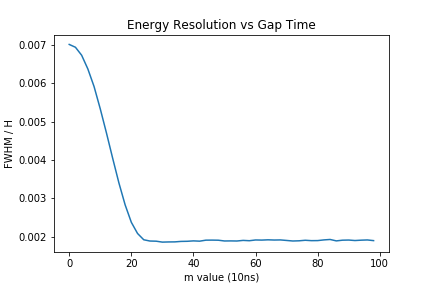
\includegraphics[width=0.7\linewidth]{images/RvsM.png}
\caption{ gap time, m, vs Energy Resolution as compared to the ${60}$Co's 1332 keV peak.}
\label{fig:MvsER}
\end{figure}


\begin{figure}[!htb]
\centering
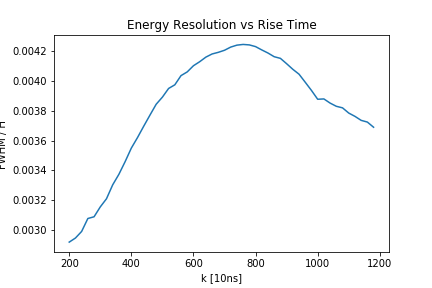
\includegraphics[width=0.75\linewidth]{images/RvsK_main.png}
\caption{ rise time, k, vs Energy Resolution as compared to the simulated pulse peak.}
\label{fig:kvsER}
\end{figure}


While Figure \ref{fig:MvsER} looks acceptable, Figure \ref{fig:kvsER} has the appearance of being inverted. This is disscused further in Section ~\ref{sec:dis}. 
The optimized m value was 30 +/-2 and the used k value was 740 +/- 20.
Additionally, the decay time was found to be 5810.2.

\subsection{Data Signals}
The following are five examples of signals from the 57Co data set before and after being put through the filter:

\begin{figure}[!htb]
\centering
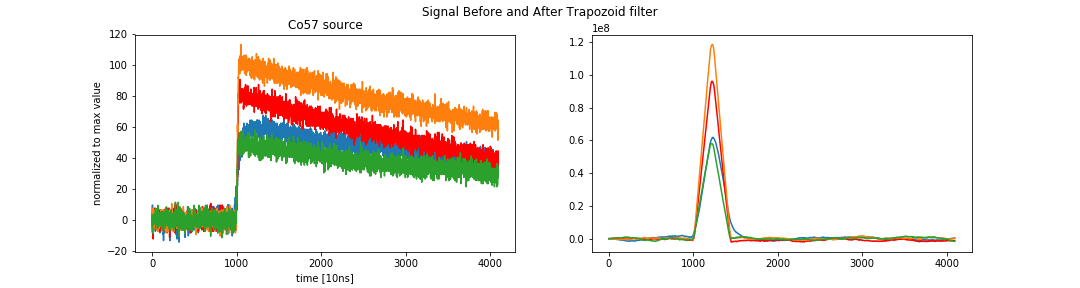
\includegraphics[width=1.0\linewidth]{images/5signals_3.png}
\caption{ Left: Raw Data signals from the SIS3302. Right: Same signals after going through the optimized trapizoidal filter.}
\label{fig:signals}
\end{figure}


\subsection{Energy Spectrum}
The following are the final energy spectra with the energy calibration done:

\begin{figure}[!htb]
\centering
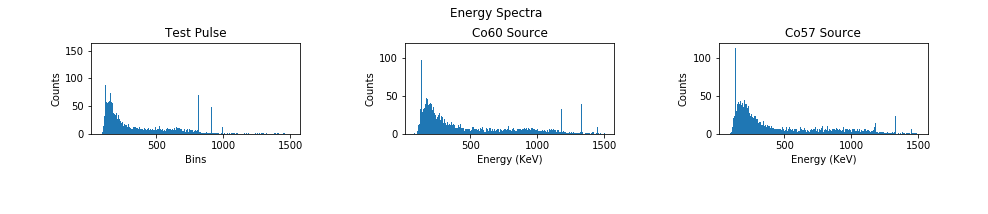
\includegraphics[width=1.0\linewidth]{images/BinnedData_3_energy.png}
\caption{ From left to right: Test Pulse Spectrum, Co57 Spectrum, Co60 Spectrum}
\label{fig:EngSpec}
\end{figure}




A discovered issue with these data set was the intense background contribution from other sources. This is discussed further in Section ~\ref{sec:dis}.


The peak selection and fitting procedure outlined in Section~\ref{sec:meth}, resulted in a linear energy calibration of the form
\begin{equation}
E = 0.1731*Bin + 82.76
\end{equation}


The energy resolution of the 3 peaks are as follows:


\begin{table}[H]
        \begin{center}
                \begin{tabular}{l|r}
                        \textbf{Peaks} & \textbf{Energy Resolution}\\
                        \hline
                        136.47      &       0.27     \\
                        1173.22     &       0.0104   \\
			1332.49     &       0.0078   \\ 
                \end{tabular}
                \caption{Energy Resolution for one 57Co peak and two 60Co peaks}
                \label{tab:CalSrc}
        \end{center}
\end{table}
